\chapter{Atividades Desenvolvidas}\label{sec:ativ_desenvolvidas}
Nesta seção, é apresentada, em detalhes, cada uma das principais atividades realizadas para a condução deste projeto.

\section{Estudo sobre Aprendizagem móvel}\label{sec:estudos_ap_movel} 
Existem várias definições de \textit{m-learning}. Ao longo dos anos, pesquisadores se dispuseram a estudar o assunto e tentaram achar uma definição. De acordo com \cite{Quinn2000}, \textit{m-learning} é um modelo de aprendizagem eletrônica (\textit{e-learning}) que utiliza equipamentos computadorizados: \textit{Palmtops}, dispositivos que rodam Windows Embedded Compact e até um telefone celular.
Em 2011, \cite{hwang2011research} disseram que uma definição amplamente aceita de \textit{m-learning} é simplesmente ``usar tecnologias móveis para facilitar o aprendizado''. Dentre outras definições, a adotada para esse projeto foi a seguinte: qualquer fornecimento educacional onde a tecnologia dominante é portátil ou dispositivos \textit{palmtop} \citep{traxler2005defining}.

Todavia, independente da definição tomada, torna-se necessário analisar vantagens e desvantagens de utilizar dispositivos móveis. De acordo com \cite{RICHAMEHTA2016} destacam-se como vantagens: (i) PDAs ou tablets com anotações e e-books são mais leves e menos volumosos que mochilas cheias de papéis, livros e até laptops; (ii) É mais fácil acomodar dispositivos móveis em uma sala se comparado à computadores de mesa; (iii) Dispositivos móveis podem ser usados em qualquer lugar e em qualquer momento, como em trens, em casa, em hotéis. Isto tem um valor inestimável para a educação \citep{CarmaMaia2008}.

De acordo com \cite{RICHAMEHTA2016}, destacam-se as seguintes desvantagens: (i) Celulares pequenos e telas de PDAs limitam-se a quantidade e tipo de informação que pode ser exibida; (ii) Baterias precisam ser recarregadas regularmente, e dados podem ser perdidos caso não se faça o carregamento correto; (iii) É difícil usar gráficos que possuem movimento, especialmente em celulares pequenos.

Devido ao processo de envelhecimento, limitações e desafios podem ser potencializadas no caso de usuários idosos, visto que podem ocorrer mudanças para o idoso durante esse processo. Além disso, é necessário que as aplicações educacionais móveis levem em consideração propostas pedagógicas adequadas e específicas para esse público. Desse modo, é indispensável que o desenvolvimento dessas aplicações seja realizado de maneira clara e objetiva, possibilitando melhor aprendizagem por parte do idoso.

\section{Levantamento e estudo dos conceitos e tecnologias para desenvolvimento de aplicações móveis}

Nesta seção serão abordados os principais conceitos relacionados ao desenvolvimento de aplicações móveis. Desse modo, os principais temas foram: (i) estudo sobre Scrum e Requisitos que trata sobre a metodologia de desenvolvimento adotada neste projeto; (ii) estudos sobre React Native que contempla o levantamento e pesquisa da tecnologia adotada para concepção do sistema; (iii) por fim, estudos sobre UI/UX que discute o conhecimento relacionado a interface e experiência do usuário.

\subsubsection{Estudos sobre Scrum e Requisitos} 
Em 2001, um grupo de 17 pessoas se reuniu para discutir a respeito de desenvolvimentos mais leves de software, pois acreditavam que os modelos em voga eram lentos e burocráticos. O resultado foi o Manifesto Ágil \citep{agileManifesto}, em que os participantes propuseram princípios a serem seguidos. Segundo os criadores, deveria haver a valorização de: (i) Indivíduos e interações mais que processos e ferramentas; (ii) Software em funcionamento mais que documentação abrangente; (iii) Colaboração com o cliente mais que negociação de contratos; (iv) Responder a mudanças mais que seguir um plano.

Dentre os artefatos do \textit{Scrum}, devem ser citados o \textit{Product Backlog} e o \textit{Sprint Backlog}. O \textit{Product Backlog} possui todas as funcionalidades necessárias para o funcionamento do produto, as quais são ordenadas por prioridade. Já o \textit{Sprint Backlog} reúne as funcionalidades que serão desenvolvidas na atual \textit{Sprint} em execução.

Os eventos do Scrum são: (i) Sprint; (ii) Reunião de Planejamento da Sprint; (iii) Reunião Diária; (iv) Revisão da Sprint; (v) Retrospectiva da Sprint.

A \textbf{\textit{Sprint}} é essencial para o Scrum, durante um período de 2 a 4 semanas são desenvolvidas as atividades do \textit{Sprint Backlog}, as quais foram previamente selecionadas do \textit{Product Backlog}. Estas atividades são escolhidas na \textbf{Reunião de planejamento da \textit{Sprint}}. É importante destacar que concomitantemente à Sprint são realizadas \textbf{Reuniões diárias}, que possuem o objetivo de reunir o time de desenvolvimento a fim de sincronizar as atividades e criar um plano para as próximas 24 horas. Ao final do período separado para o incremento do produto, ocorre a \textbf{Revisão da Sprint}, com o objetivo de discutir o que foi feito, inspecionar o incremento e adaptar o \textit{Product Backlog}. A \textbf{Retrospectiva da Sprint} ocorre depois da Revisão da Sprint e antes da Reunião de planejamento da próxima Sprint, e é a oportunidade para o Time Scrum inspecionar a si próprio criar um plano para melhorias a serem aplicadas na próxima Sprint.

Ademais, existem funções diferentes para os membros chamadas de papéis. São eles: \textit{Product Owner}; Time de Desenvolvimento e \textit{Scrum Master}. 
O \textit{Product Owner}, ou dono do produto, se encarrega de maximizar o valor do produto e gerenciar os \textit{Backlogs}. O Time de Desenvolvimento concentra os profissionais responsáveis pelos incrementos do produto. Por fim, o \textit{Scrum Master} orquestra toda a equipe e deve garantir que o Scrum seja entendido e aplicado.

Outro fator importante para o desenvolvimento de um software são os requisitos. De acordo com \cite{Sommervile2010}, eles podem ser definidos como os serviços que o sistema promove, as restrições de operação e as descrições do que o sistema deveria realizar. É importante destacar a Engenharia de Requisitos, a qual fornece mecanismos apropriados para o entendimento da demanda do consumidor, análise de suas necessidades, avaliação da viabilidade, negociação de uma solução, especificação de uma solução não ambígua, validação da especificação e gerenciamento de requisitos enquanto são transformados em um sistema operacional \citep{Pressman2014}. 

Três são os principais tipos de requisitos \citep{Sommervile2010}:
\begin{itemize}
    \item \textbf{Requisitos funcionais}: são declarações de serviços que o sistema deve prover, como o sistema deve reagir a determinados tipos de entrada, e como deveria funcionar em situações particulares. Em alguns casos, os requisitos funcionais podem também explicitar o que o sistema não deveria fazer.
    
    \item \textbf{Requisitos não funcionais}: são restrições dos serviços ou funções oferecidos pelo produto. Incluem restrições de tempo, de processos de desenvolvimento, e restrições impostas por padrões. Requisitos não funcionais frequentemente se aplicam ao sistema como um todo, em vez de se aplicar a serviços ou \textit{features} individuais.
    
    \item \textbf{Requisitos de domínio}: são derivados do domínio de aplicação do sistema, e não de necessidades específicas de usuários do sistema. Podem ser novos requisitos funcionais, restringindo os já existentes. 
\end{itemize}


\subsection{Estudos sobre React Native} 
São diversas as maneiras de desenvolver um aplicativo móvel. A maneira convencional é utilizar a linguagem nativa: Java (Android) e Swift/Object-C (iOS), todavia isso causa o empecilho de se disponibilizar o aplicativo apenas para uma plataforma. Ainda, é possível usar \textit{frameworks} híbridos que recorrem ao uso de \textit{web-views} para renderizar a aplicação e disponibilizar para os dois sistemas operacionais, pode-se citar Ionic, Titanium, e PhoneGap. Entretanto, o desempenho de aplicativos construídos com tais tecnologias é precário. Pensando no problema, durante a conferência do React.js em 2015, o Facebook introduziu seu novo \textit{framework} React Native, o qual prometia revolucionar a maneira de desenvolver aplicativos móveis. A premissa era simples, possibilitar o desenvolvimento \textit{mobile} sem a necessidade de programação diferente para os dois sistemas operacionais líderes.

% Vantagens e desvantagens
As principais vantagens do uso do React Native, de acordo com \cite{danielsson2016}, são: (i) O desenvolvimento ocorre em uma única linguagem, sendo possível utilizar o aplicativo em iOS ou Android; (ii) A documentação oficial dá grande suporte de ajuda; (iii) O React Native não possui nenhum efeito negativo na experiência do usuário, pois a diferença de desempenho é imperceptível para a grande maioria dos usuários.

Dentre as desvantagens, é importante destacar: (i) Incerteza da possibilidade de executar frequentes tarefas em segundo plano quando o aplicativo já está sendo executado em segundo plano \citep{sodebergJohansson}; (ii) Testes concluem que a frequência GPU, carregamento de CPU, uso de memória e consumo de energia são levemente inferiores ao desenvolvimento nativo \citep{danielsson2016}.

Entretanto, embora existam algumas desvantagens do uso do React Native, em termos gerais é uma excelente alternativa para o projeto, pois não compromete de maneira significante a performance do aplicativo e possibilita o uso nas plataformas iOS e Android, alcançando assim, um número maior de usuários.

\subsection{Estudos sobre UI/UX}
A Interface de Usuário (UI) se refere a um sistema e um usuário interagindo um com outro por meio de comandos para operar o sistema, inserir dados, e usar o conteúdo \citep{joo2015}. Já a Experiência de Usuário (UX), segundo \cite{marc2008}, é uma perspectiva distinta da qualidade de tecnologia interativa. O autor ainda define UX como uma avaliação momentânea e primária da sensação (bom-ruim) enquanto interage com o produto ou serviço. Dessa forma, UX troca a atenção dos produtos e materiais para as sensações humanas - o lado subjetivo do uso do produto. Ainda, de acordo com \cite{castilla2017}, a UX representa uma mudança do próprio conceito de usabilidade, pois o objetivo não se reduz a melhorar a sensação do usuário na eficácia, eficiência e facilidade de aprendizagem, mas sim tentar resolver o problema estratégico da utilidade do produto para o usuário. 

Dessa maneira, pode-se concluir que a interface e experiência do usuário cumprem papéis essenciais no desenvolvimento de um produto, sendo indispensável seu planejamento. Ainda, tendo em vista o público alvo do atual projeto, usuários idosos, torna-se necessária a atenção e cuidado no assunto a fim de alcançar os objetivos finais.

Portanto, tendo em mente os motivos acima citados, foi realizado um minicurso sobre a Experiência de usuário e Interface de usuário com uma especialista da área UI/UX cujo título era ``Como incluir UX e UI Design nos seus projetos''. A realização se deu na 22ª Semana da Computação da Universidade de São Paulo, campus de São Carlos, no dia 03/10. O minicurso se mostrou de grande importância, uma vez que possibilitou a expansão do conhecimento do assunto em termos práticos, sendo possível sua aplicação no projeto.

\section{Pesquisa sobre as principais funcionalidades de aplicativos de aprendizagem móvel} 
Diversos são os aplicativos que possuem o objetivo de apoiar o processo de ensino e aprendizagem do usuário; seja por meio de jogos, vídeos ou outros materiais. Dessa maneira, alguns aplicativos (para diferentes públicos) foram analisados, a fim de verificar suas funcionalidades e propostas de aprendizagem e acessibilidade, de maneira que essas pudessem ser adaptadas ou utilizadas para aplicações com foco no idoso.

\begin{description}
% Ensina o que? Qual o publico alvo? Pessoas de quantos anos?

\item[Engaging congress]\footnote{\url{https://play.google.com/store/apps/details?id=com.iu.engagingcongress&hl=en}, \url{https://apps.apple.com/us/app/engaging-congress/id1309161238?ls=1}} \hfill \\
\textit{Enganging congress} (\autoref{fig:EngCong}) é um jogo interativo que visa explorar os princípios básicos de um governo representativo. Escolhe-se um tema e é exibido um vídeo. Jogos são incluídos no processo baseados no tema. É importante destacar a atenção dos criadores em fazer o usuário compreender a tarefa; a todo momento é possível clicar no botão de dúvida. As principais funcionalidades são: (i) vídeos educativos sobre o tema; (ii) perguntas relacionadas ao conteúdo passado; (iii) nota final após a conclusão dos exercícios; (iv) botões de dúvidas sempre presentes.

\begin{figure}[ht!]
\centering
    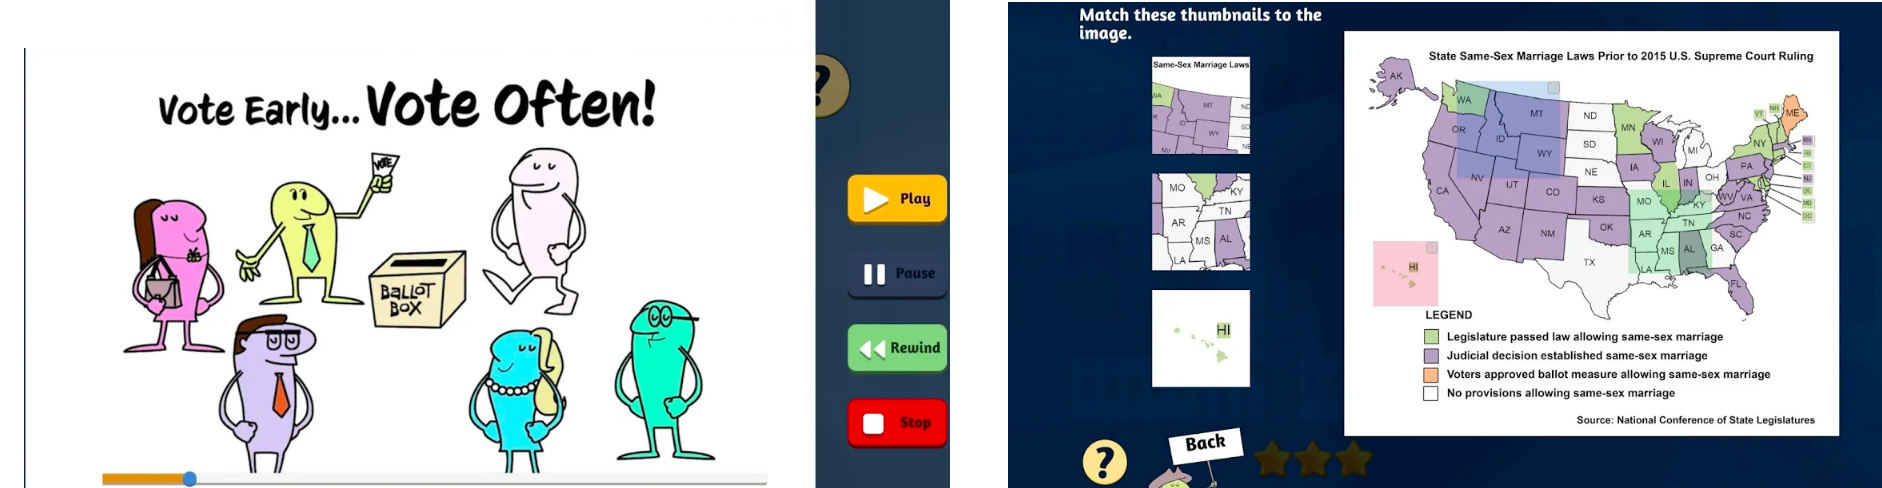
\includegraphics[width=0.9\textwidth]{Figuras/engagingcongress.png}
    \caption{Telas do aplicativo \textit{Engaging Congress}}
    \label{fig:EngCong}
\end{figure}

\item[Play PBS KIDS Games]\footnote{\url{https://apps.apple.com/us/app/pbs-kids-games/id1050773989}, \url{https://play.google.com/store/apps/details?id=org.pbskids.gamesapp&hl=pt_BR}} \hfill \\
O aplicativo (\autoref{fig:pbs}) visa a promoção da educação para crianças na fase de alfabetização (2 a 8 anos), pois contém mais de 100 mini-jogos voltados para tal. As crianças são encorajadas a resolver desafios e aprimorar suas habilidades em ciências, matemática, letras e criatividade. O objetivo é impactar positivamente as vidas de crianças por meio de mídia baseada em um currículo onde quer que elas estejam. O app ganhou duas premiações no ano de 2017, a saber Melhor aplicativo de jogos para Pré-Escola (\textit{Kidscreen Award Winner}) e o \textit{Parents' Choice Recommended Mobile App}. Os principais recursos são: (i) funcionamento offline; (ii) possibilidade de gerenciar a quantidade de memória que será consumida; (iii) obter detalhes sobre desenhos da TV PBS Kids como idade recomendada e objetivos de aprendizado para as crianças.

\begin{figure}[H]
\centering
    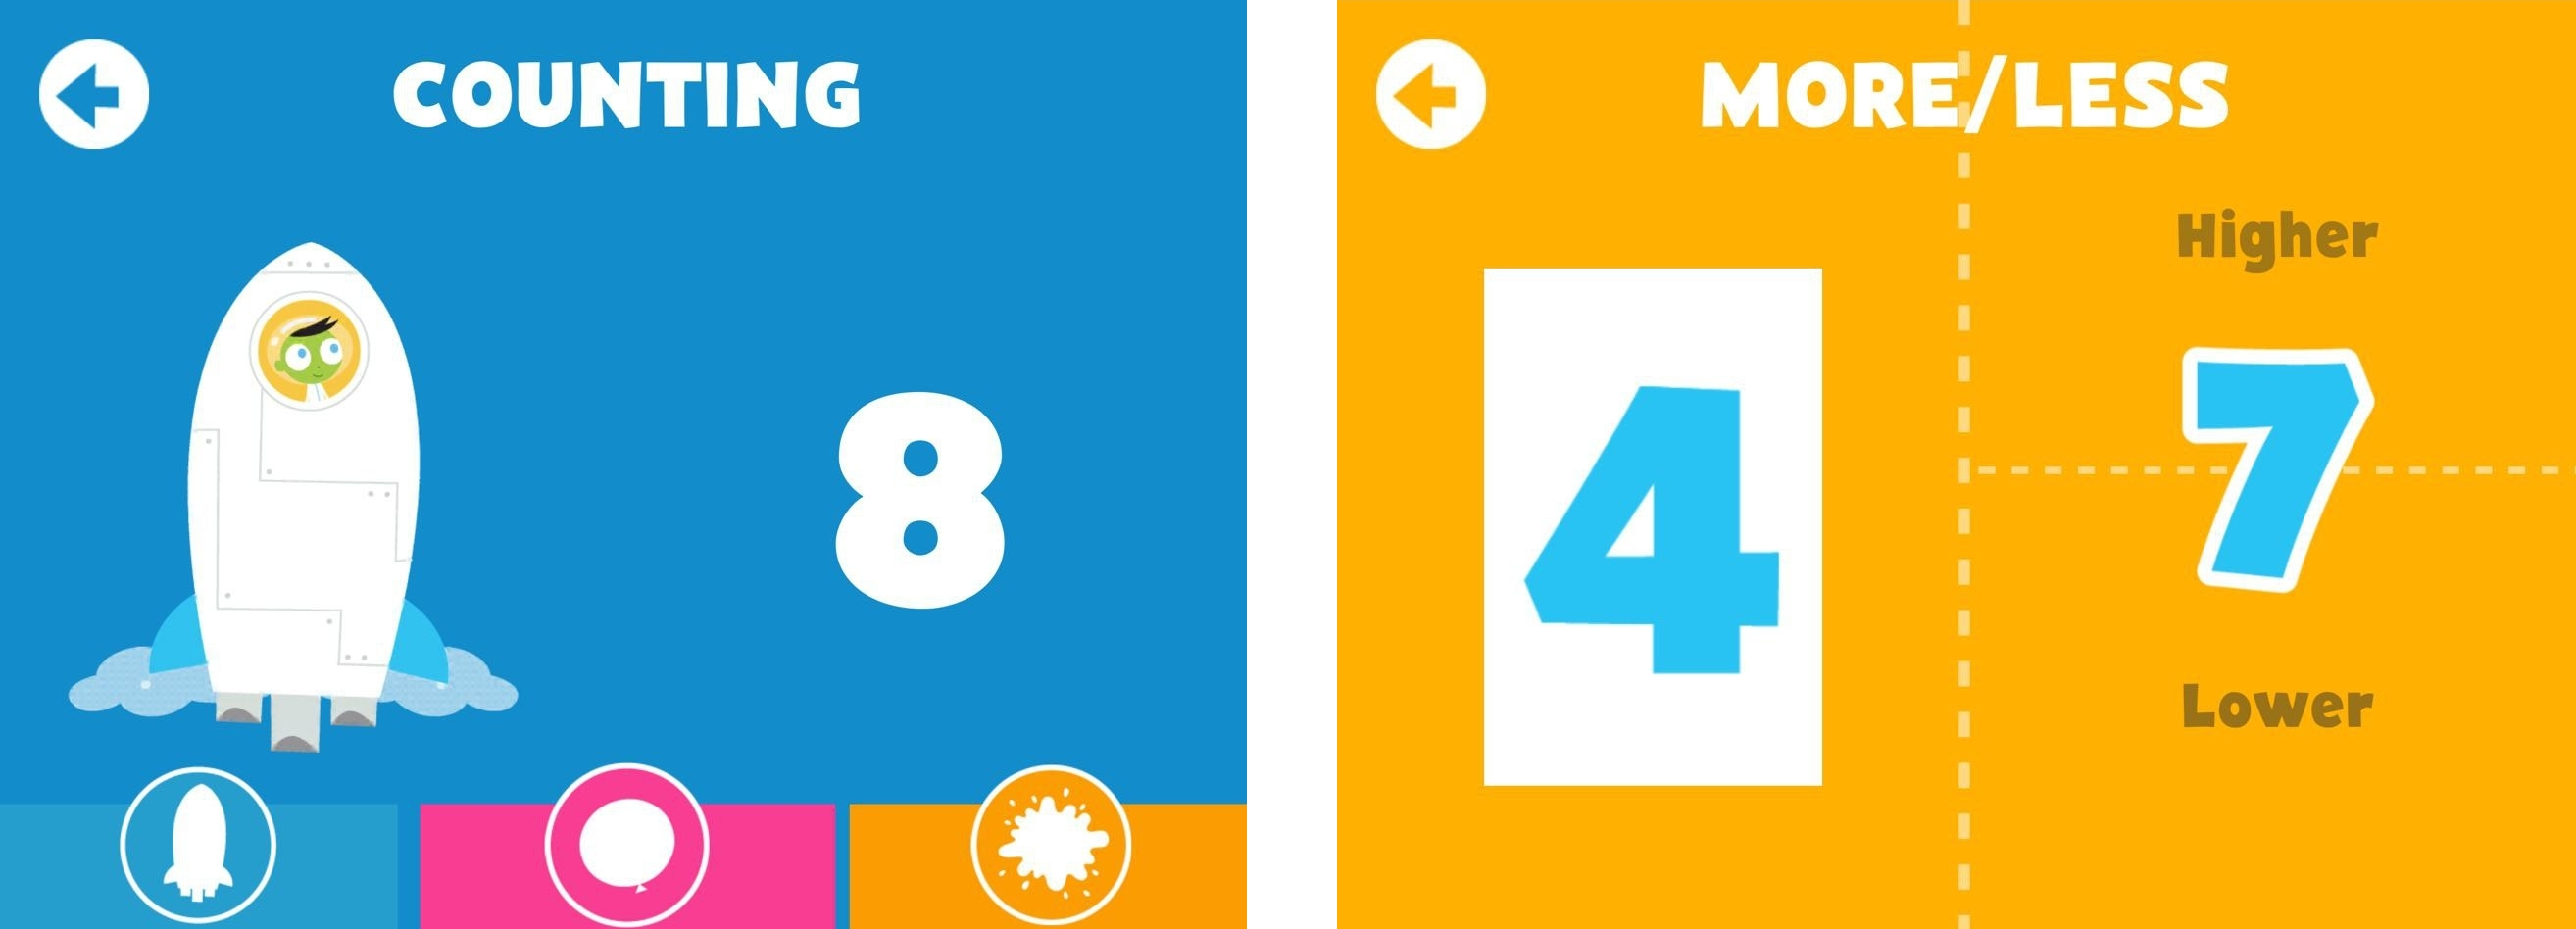
\includegraphics[width=0.9\textwidth]{Figuras/pbsKids.jpg}
    \caption{Telas do aplicativo \textit{Play PBS KIDS Games}}
    \label{fig:pbs}
\end{figure}

\item[Human Anatomy Atlas]\footnote{\url{https://apps.apple.com/br/app/human-anatomy-atlas-2020/id1117998129}, \url{https://play.google.com/store/apps/details?id=com.argosy.vbandroid&hl=pt_BR}} \hfill \\
O \textit{Human Anatomy Atlas} (\autoref{fig:humAtlas}) é um aplicativo criado por um time de especialistas em visualização biomédica. É direcionado ao ensino da anatomia do corpo humano com o foco em estudantes e professores, apesar de também ser utilizado em hospitais. Seus modelos em 3D promovem uma fidelidade às estruturas humanas reais, sendo possível rotacionar e dissecar órgãos e partes do corpo. Possui recursos como : (i) interatividade com estruturas 3D; (ii) mais de 1000 questões para testes em assuntos; (iii) visualização de anatomias complexas em realidade aumentada; (iv) disponibilidade em 7 idiomas.

\begin{figure}[ht!]
\centering
    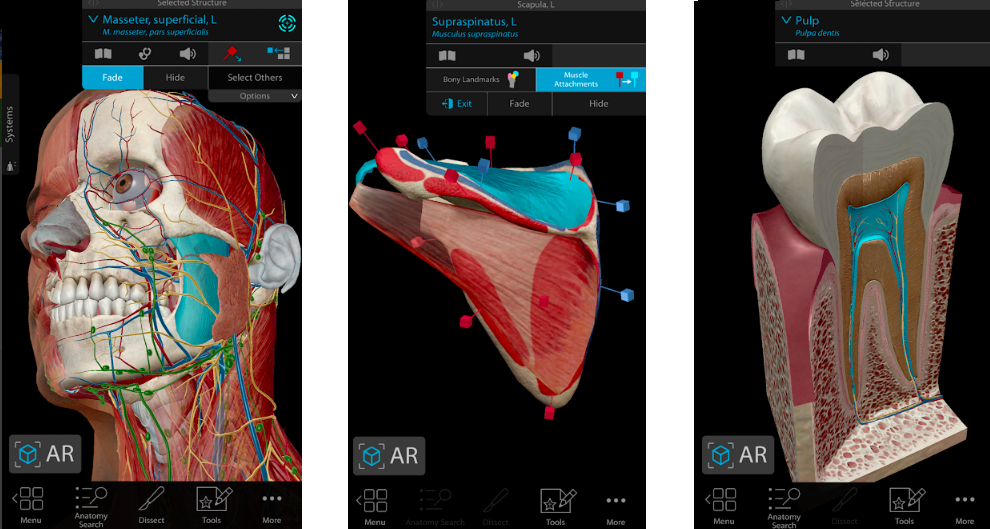
\includegraphics[width=0.9\textwidth]{Figuras/humanAtlas.png}
    \caption{Telas do aplicativo \textit{Human Anatomy Atlas}}
    \label{fig:humAtlas}
\end{figure}

\item[Bini Super ABC]\footnote{\url{https://apps.apple.com/br/app/bini-abc-alfabeto-crianças-app/id1397966958}, \url{https://play.google.com/store/apps/details?id=com.binibambini.abc&hl=pt_BR}} \hfill \\
Bini Super ABC (\autoref{fig:biniABC}) é um aplicativo voltado para crianças na faixa de 3 a 5 anos na fase de instrução educacional. O aplicativo promove o aprendizado das letras do alfabeto com diversos jogos infantis. O objetivo é tornar o ensino interessante e empolgante com desenhos coloridos, personagens e efeitos sonoros. A aplicação possui as funcionalidades: (i) aprendizado das letras por sons; (ii) reforço do material aprendido; (iii) controle de responsáveis para os jogos.

\begin{figure}[H]
\centering
    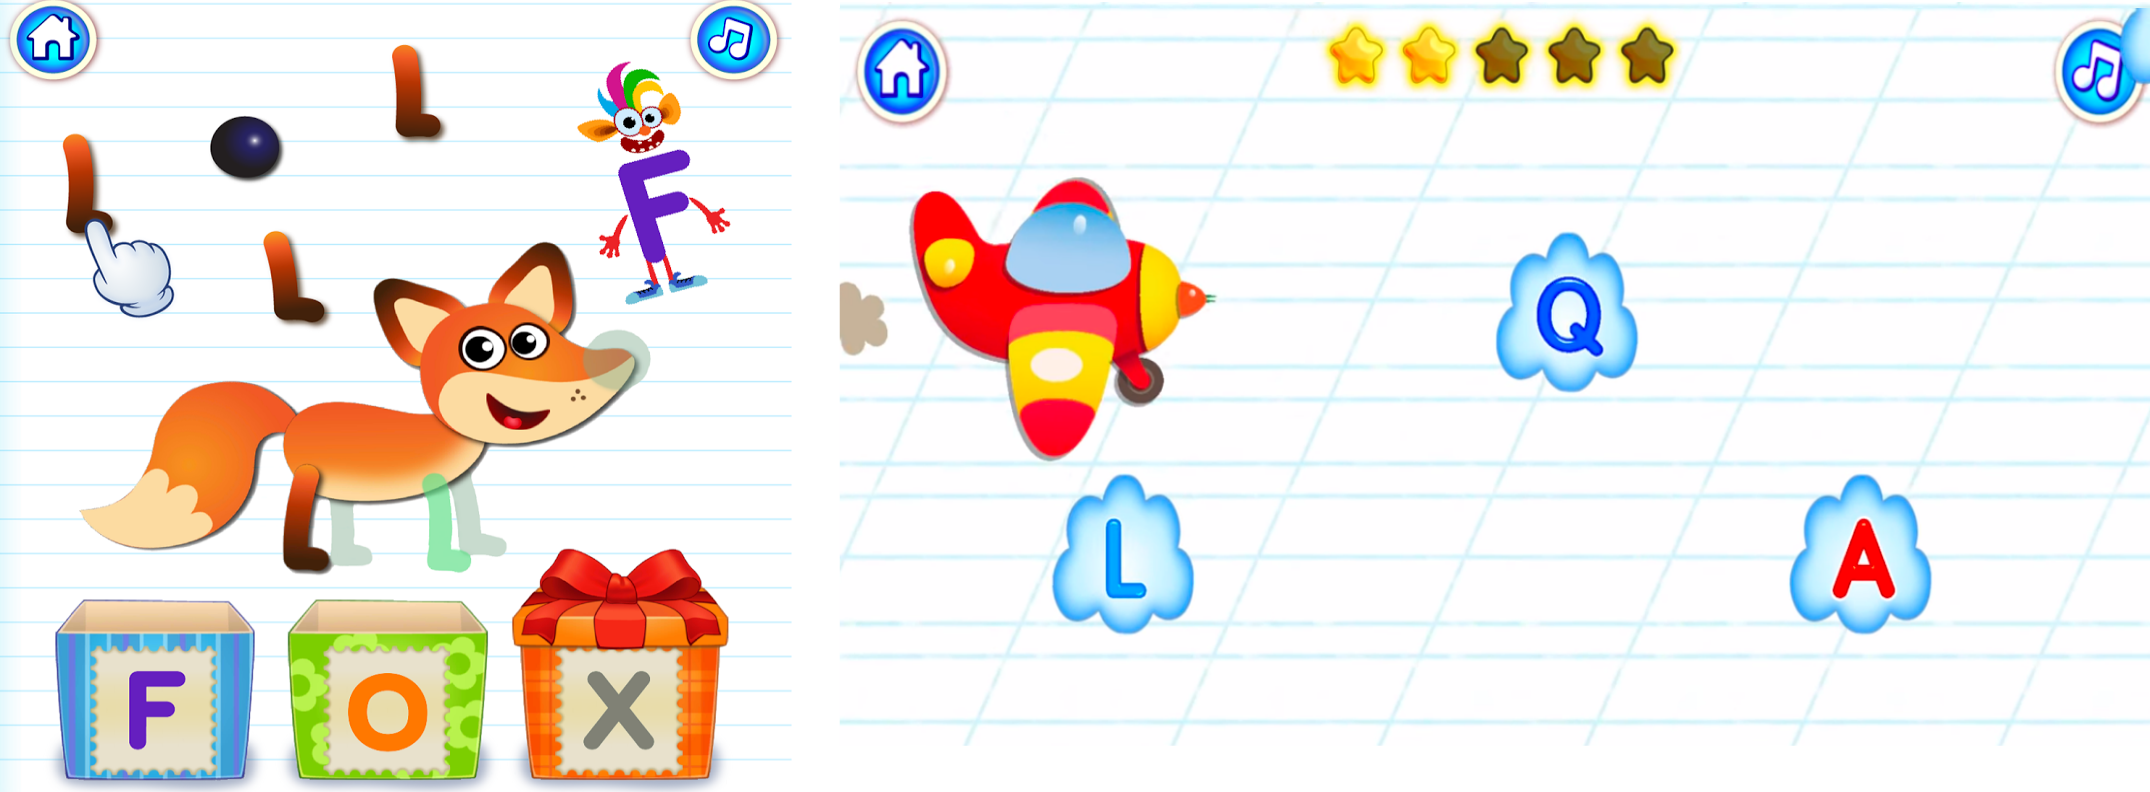
\includegraphics[width=0.9\textwidth]{Figuras/biniabc.png}
    \caption{Telas do aplicativo \textit{Bini Super ABC}}
    \label{fig:biniABC}
\end{figure}

\item[Crossword Puzzle Free]\footnote{\url{https://play.google.com/store/apps/details?id=mobi.redstonegames.crossword.en&hl=pt_BR}} \hfill \\
Crossword Puzzle Free (\autoref{fig:crossFree}) é um aplicativo de palavras cruzadas. É simples e fácil de usar não exigindo conhecimentos específicos do usuário. Com os 4 níveis de dificuldade é possível buscar o desafio na medida certa além de motivar o usuário a continuar utilizando o aplicativo por não ser nem muito fácil nem muito difícil. As principais funcionalidade são: (i) Teclado do próprio aplicativo; (ii) Dicas aparecem acima do teclado; (iii) Botão de dica para a palavra.


\begin{figure}[H]
\centering
    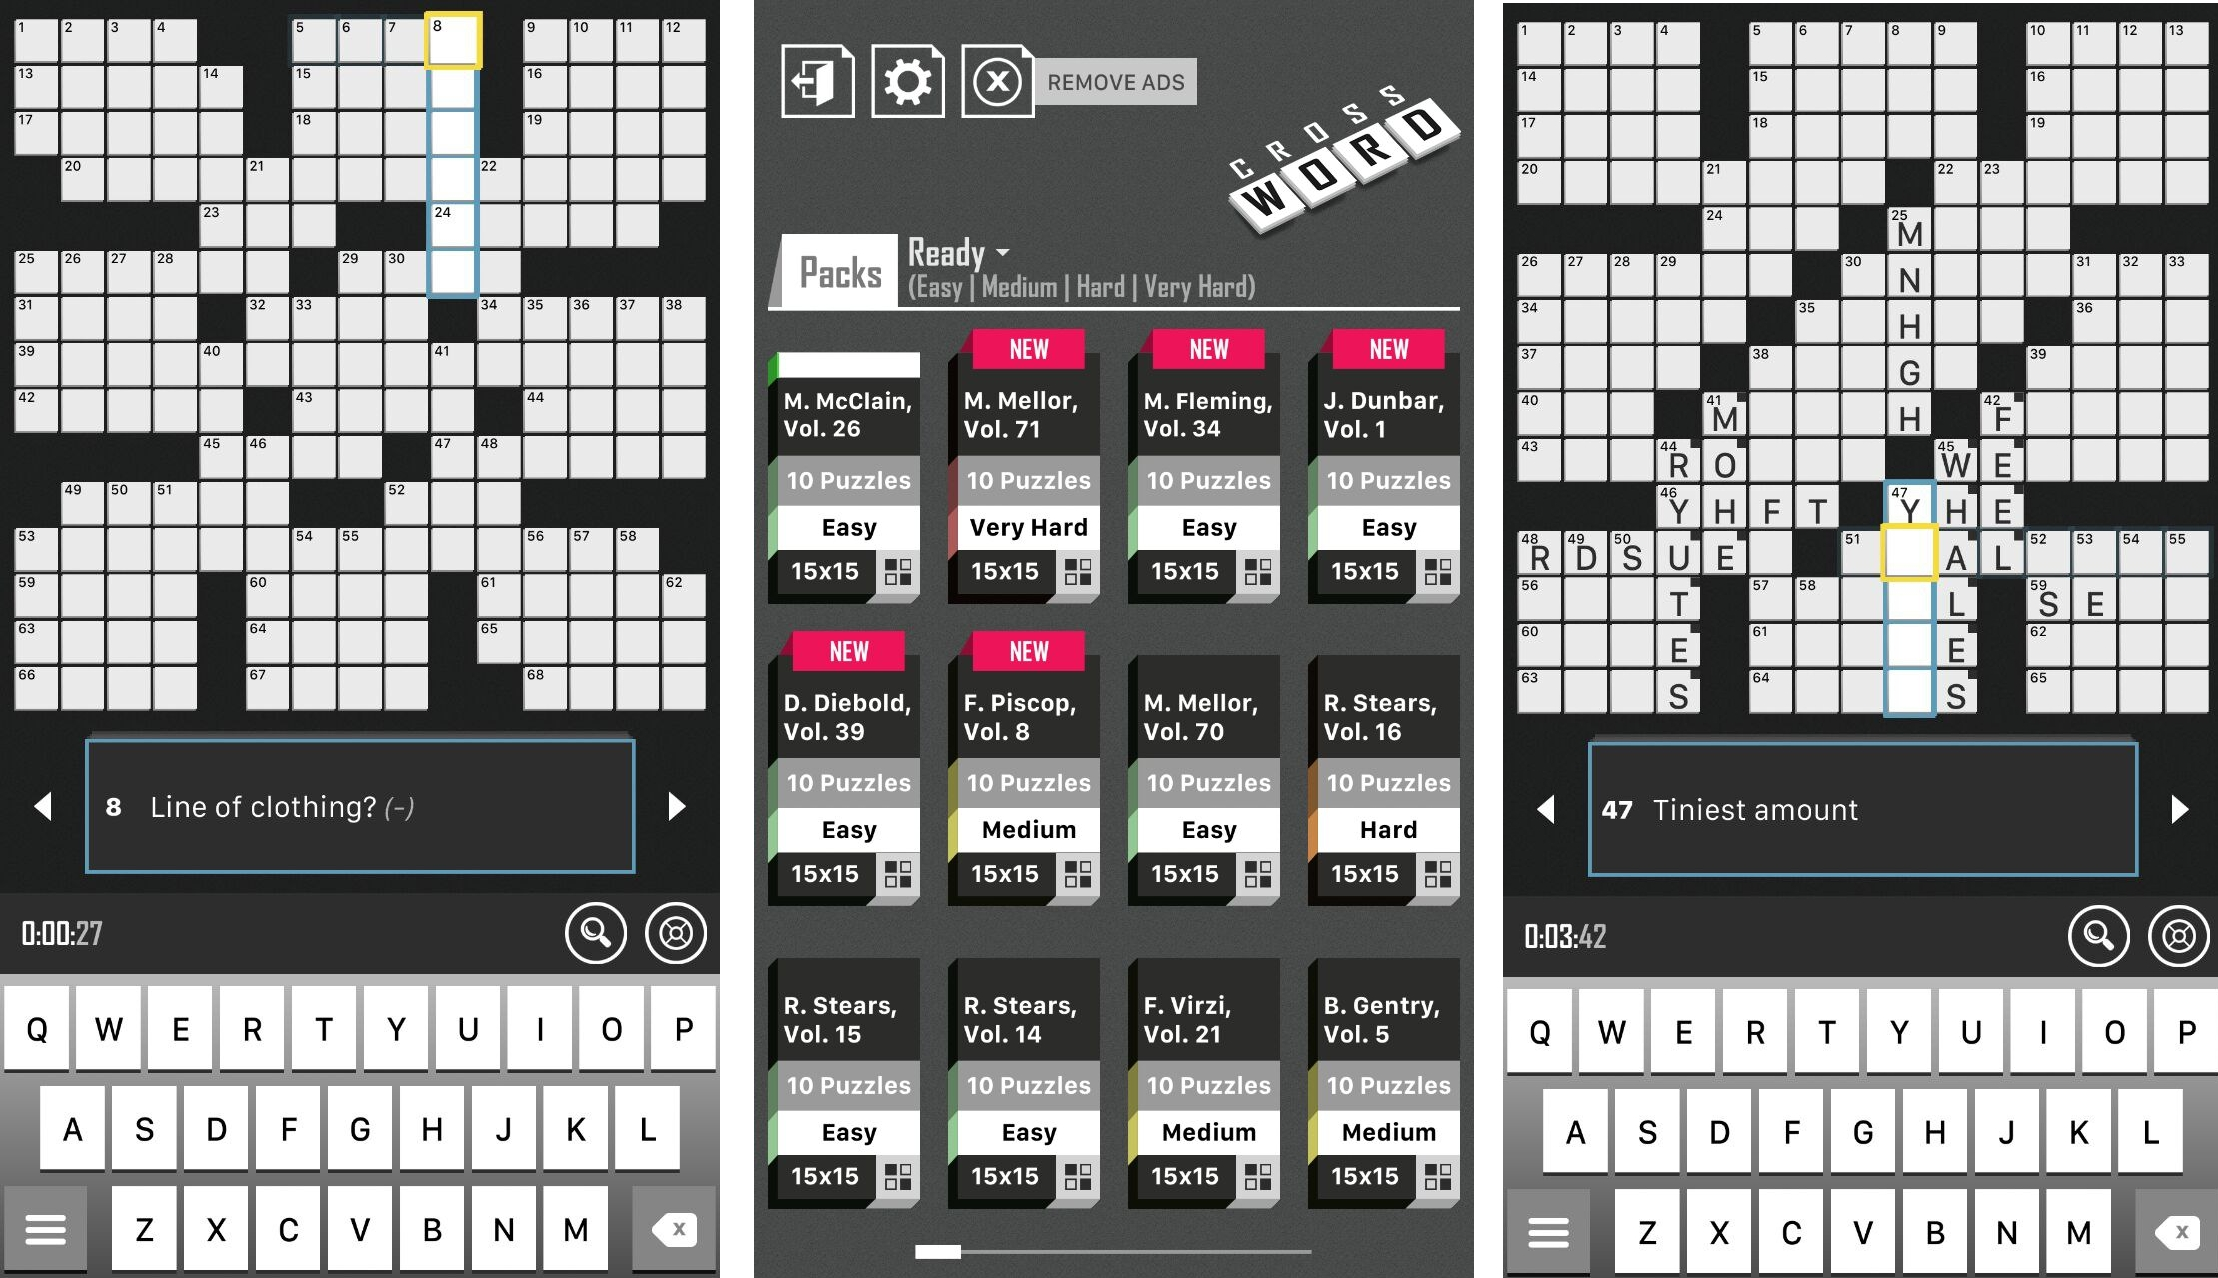
\includegraphics[width=0.9\textwidth]{Figuras/crosswordPuzzleFree.jpg}
    \caption{Telas do aplicativo \textit{Crossword Puzzle Free}}
    \label{fig:crossFree}
\end{figure}

\item[Crossword Quiz]\footnote{\url{https://play.google.com/store/apps/details?id=com.randomlogicgames.crossword&hl=pt_BR}} \hfill \\
Crossword Quiz (\autoref{fig:crossQuiz}) é um aplicativo de palavras cruzadas com uma abordagem mais fácil por não disponibilizar todas as letras do teclado, tornando a resposta mais fácil para o usuário. Além disso, o aplicativo não conta apenas com dicas escritas, mas inclui imagens. As funcionalidade que se destacam são: (i) Não mostrar todo o teclado, apenas algumas letras; (ii) Mostra imagens como dicas além de textos; (iii) Tutorial inicial intuitivo e completo.

\begin{figure}[H]
\centering
    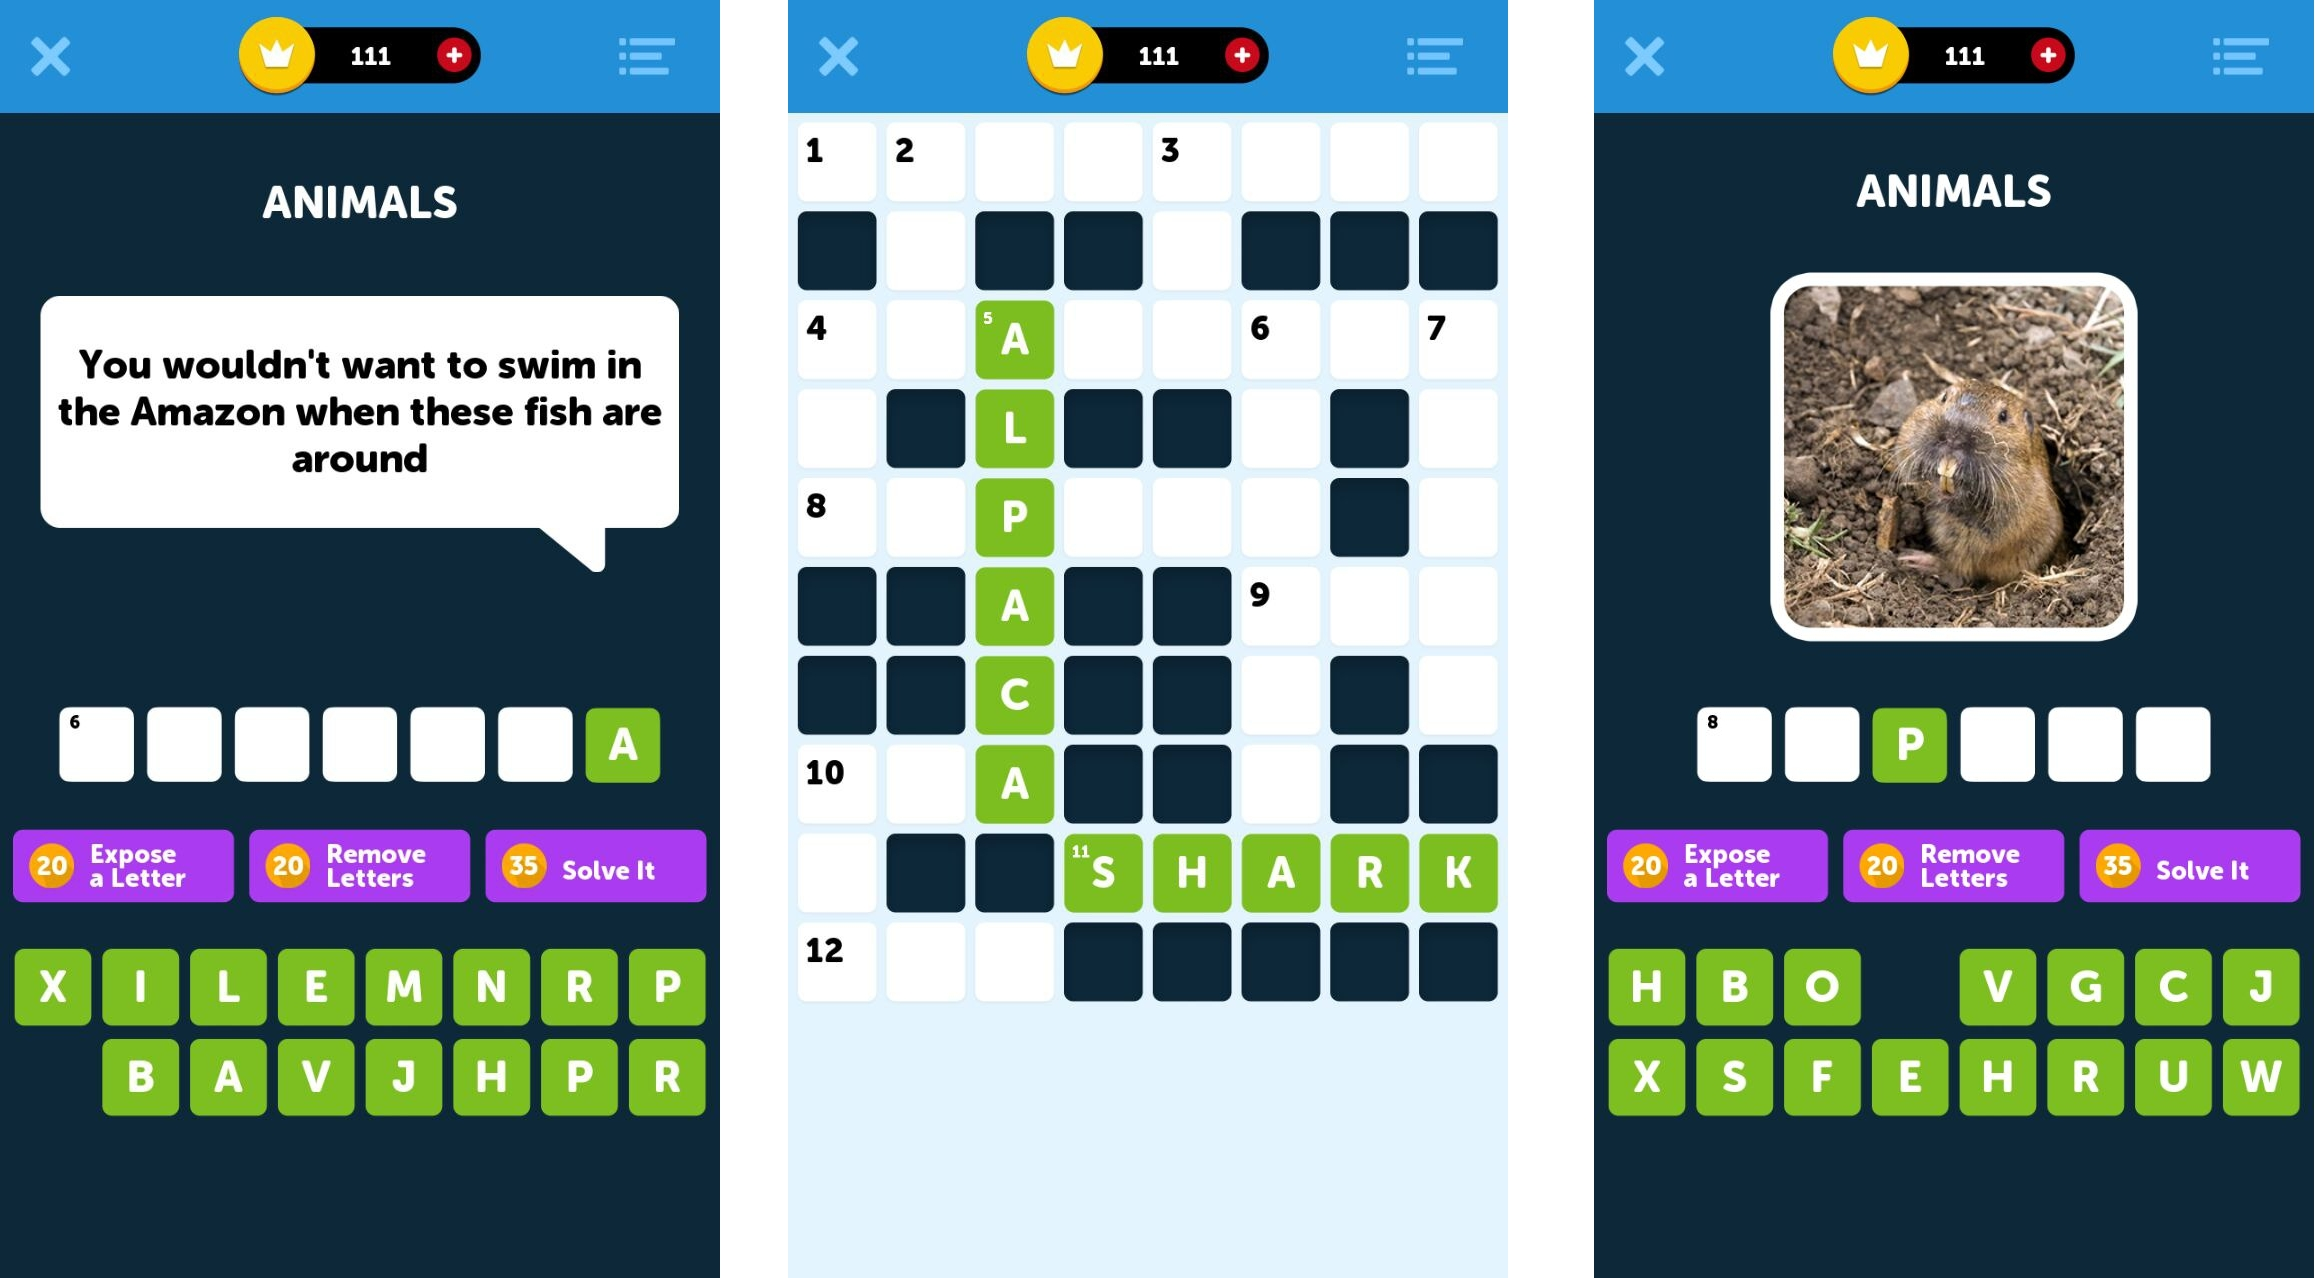
\includegraphics[width=0.9\textwidth]{Figuras/crosswordQuiz.jpg}
    \caption{Telas do aplicativo \textit{Crossword Quiz}}
    \label{fig:crossQuiz}
\end{figure}

\end{description}



\begin{table}[!ht]
\caption{\textit{Funcionalidades das aplicações educacionais}}
\centering
\footnotesize
\begin{tabular}{p{6cm} p{12cm}}
\toprule
\textbf{Aplicativo} & \textbf{Funcionalidades}                                              \\ \midrule

Engaging congress   & \begin{tabular}[c]{@{}l@{}}Vídeos educativos\\ Perguntas relacionadas ao conteúdo\\ Nota após término dos exercícios\\ Botões de dúvida em todas as telas\end{tabular}                                                                 \\ \midrule
Play PBS KIDS Games & \begin{tabular}[c]{@{}l@{}}Funcionamento offline\\ Gerenciamento de consumo de memória\\ Obtenção de detalhes de desenhos passados na TV PBS Kids\end{tabular}      \\ \midrule
Human Anatomy Atlas & \begin{tabular}[c]{@{}l@{}}Interatividade com estruturas 3D\\ Mais de 1000 questões para testes\\ Realidade aumentada\\ Sete idiomas disponíveis\end{tabular}    \\ \midrule
Bini Super ABC & \begin{tabular}[c]{@{}l@{}}Aprendizado das letras por sons\\ Reforço do material aprendido\\ Controle de responsáveis para jogos\end{tabular}                \\ \midrule
Crossword Puzzle Free & \begin{tabular}[c]{@{}l@{}}Teclado próprio\\ Dica acima do teclado\\ Botão de dica para a palavra\end{tabular}                \\ \midrule
Crossword Quiz & \begin{tabular}[c]{@{}l@{}}Não mostra o teclado todo, apenas algumas letras\\ Mostra imagens em vez de dicas em texto também\\ Tutorial inicial mostrando todos os passos antes de mesmo de permitir o jogador jogar uma partida sozinho\end{tabular}                \\ \midrule
\end{tabular}
\label{tab:sprint}
\end{table}



\section{Estudo do algoritmo de geração das palavras cruzadas} 
Nesta seção será abordado o algoritmo de geração das palavras cruzadas do aplicativo. Para melhor compreensão deste, é essencial a noção dos paradigmas clássicos da Ciência da Computação: Força Bruta e \textit{Backtracking}. Além disso, faz-se necessário uma pequena noção das Cadeias de Markov absorventes para estipulação e análise do tempo de execução do algoritmo até que se encontre uma solução. Por fim, utilizando os conceitos anteriormente explanados, será possível compreender o algoritmo com melhor profundidade.

\subsection{Força Bruta e \textit{Backtracking}}


\subsection{Cadeias de \textit{Markov}}
sooooom

\subsection{Desenvolvimento do algoritmo}
sooooom